\clearpage 
\begin{figure}[t!]
  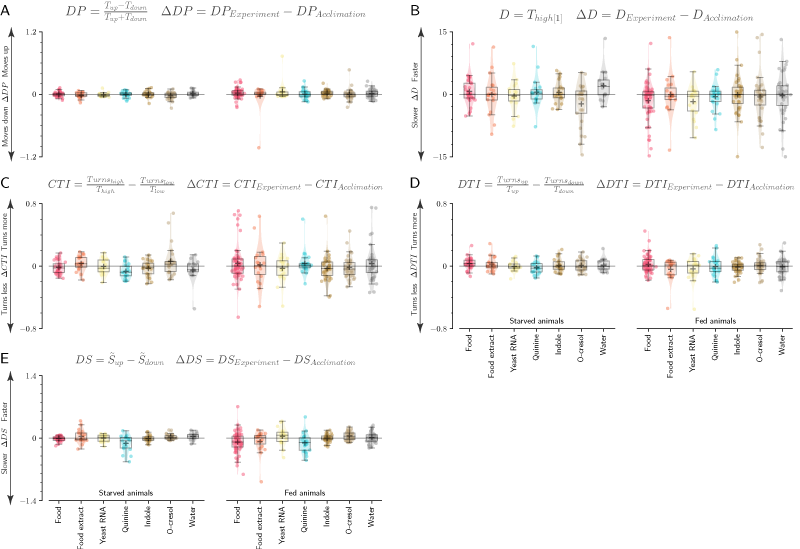
\includegraphics[width=\linewidth]{Figures/images/S3.eps}
  \caption{\textbf{Larval behavior is not consistent with chemotaxis or klinokinesis search strategy models.} A-E: Box plots for the population median (${\pm}$ 1 quartile), population mean (+ marker) and mean response for each individual (dots). We observed no significant changes across stimuli for any of these five behavioral metrics (p>0.05, Kruskal-Wallis test). A: Directional Preference ${\Delta}$DP, difference in time (${T}$) moving up or down the concentration map. B: Discovery time ${\Delta}$D, time (${T}$) elapsed before initial encounter of high concentration (${\geq}$50${\%}$). C: Concentration-dependent Turn Incidence ${\Delta}$CTI, difference in turning rate at high and low local concentrations. D: ${\Delta}$Concentration-dependent Turn Incidence ${\Delta}$DTI, difference in turning rate while moving up or down concentration.E: ${\Delta}$Concentration-dependent Speed ${\Delta}$DS, difference in mean speed (${\tilde{S}}$) while moving up or down the concentration map.}
\end{figure}
